\documentclass[11pt,a4paper]{article}
\usepackage[utf8]{inputenc}
\usepackage{graphicx}
\usepackage[table]{xcolor}
\usepackage[overlay,absolute]{textpos}
\usepackage[multiple]{footmisc}
\usepackage{fancyhdr}
\usepackage{hyperref}
\usepackage[top=35mm, bottom=35mm, left=35mm, right=30mm]{geometry}
\usepackage[style=ieee,autocite=inline,bibencoding=ascii,backend=bibtex]{biblatex}
\usepackage{xstring}
\usepackage{caption}
\usepackage{array}
\usepackage{float}
\usepackage{setspace}
\usepackage{pdflscape}
\usepackage[number]{abstract}
\usepackage{afterpage}
\usepackage{listings}
\usepackage{algpseudocode}
\usepackage{algorithm}
\usepackage{amsmath}
\usepackage{pgfgantt}
\usepackage{subcaption} 

%\singlespacing
\onehalfspacing
%\doublespacing

\fancyhf{} % clear all header and footers
\rfoot{\thepage}
\pagestyle{fancy}

% For inserting a blank page.
\newcommand{\blankpage}{
\newpage
\thispagestyle{empty}
\mbox{}
\newpage
\addtocounter{page}{-1}
}

\newcolumntype{L}[1]{>{\raggedright\let\newline\\\arraybackslash\hspace{0pt}}m{#1\textwidth}}
\newcolumntype{C}[1]{>{\centering\let\newline\\\arraybackslash\hspace{0pt}}m{#1\textwidth}}
\newcolumntype{R}[1]{>{\raggedleft\let\newline\\\arraybackslash\hspace{0pt}}m{#1\textwidth}}
\newcolumntype{P}[1]{>{\raggedright\right\newline\\\arraybackslash\hspace{0pt}}p{#1\textwidth}}

%% To prevent overfull hbox in bibliography.
\emergencystretch=1em

%%% Include bibtex references.
\addbibresource{references.bib}

\title{Final Report}
\author{Taylor Young\\Student Number: 3206230}

\begin{document}
%Title
\def\isfinalreport{1}
\begin{titlepage}
    \begin{center}
        % Upper part of the page. The '~' is needed because \\
        % only works if a paragraph has started.
        \begin{center}
            \includegraphics[width=0.15\textwidth]{./figures/uon_logo.png}
            
            \textsc{\LARGE University of Newcastle}\\[1cm]
        \end{center}
        
        % Title
        % Author and supervisor
        \begin{textblock*}{133mm}(49mm,75mm)  %% change width of box from 10in as you wish
            \begin{minipage}[t][65mm][t]{133mm}
                \centering
                ~\\[0.5cm]
                \textsc{\Large Interim Report}\\[0.5cm]
            
                \hrule ~\\[0.5cm]
                { \Large Pneumatic Muscle Joint Research and Design\\[0.5cm] }
                \hrule ~\\[0.5cm]
            
                \noindent
                \begin{minipage}{0.4\textwidth}
                    \begin{flushleft} \large
                        \emph{Author:}\\
                        Taylor \textsc{Young}\\
                        Student Number: 3206230
                    \end{flushleft}
                \end{minipage}%
                \begin{minipage}{0.4\textwidth}
                    \begin{flushright} \large
                        \emph{Supervisors:} \\
                        Colin \textsc{Coates}\\
                    \end{flushright}
                \end{minipage}\\[0.5cm]
                \hrule ~\\[0.3cm]
                {\large \today}
            \end{minipage}
        \end{textblock*}
    \end{center}
    
    \vfill
    
    \emph{A thesis submitted in partial fulfilment of the requirements for the degree of Bachelor of Engineering in Electrical (Computer or Telecommunications) Engineering at The University of Newcastle, Australia.}
    
    \vfill
\end{titlepage}

% pdflatex -synctex=1 -shell-escape Final_Report.tex
\blankpage
\pagenumbering{gobble}

%%% Use roman numerals for page numbering in document preamble (abstract, TOC, acknowledgements, etc).
\pagenumbering{roman}

%Abstract
\section*{Abstract}
\addcontentsline{toc}{section}{Abstract}
Humanoid robotics is a fast-developing field encompassing a wide range of engineering disciplines to solve the challenges of robotics interaction in an environment designed for humans. In order to encourage this development many competitions exist around very common but highly specific human tasks, all of which aim to extend the field of humanoid robotics and general intelligence. In order to walk, robots need some method of actuating joints in a controllable, fast and energy efficient way.\newline
This project is to design and construct a single leg based on a custom developed humanoid robotic platform, focusing on the knee and ankle joints specifically. A single degree of freedom test rig has been constructed to test the feasibility of both the pneumatic muscles and the control scheme.
A mathematical model for the actuator has been used to inform the control system structure and allow the estimation of the current system state. Pneumatic muscles are a highly nonlinear actuator, this means that standard linear controllers have limited success in controlling the actuator position. Control can be achieved with only a static force map leading to an accurate, high-performance control scheme, however, pneumatic muscles also have their own dynamics, like hysteresis, some thermodynamic effects. \newline
Therefore, a nonlinear MPC controller has been implemented and theoretically compared to two other controllers. \newline \newline TODO This probably needs more about muscle design
\blankpage

%Acknowledgements
\section*{Acknowledgements}
\addcontentsline{toc}{section}{Acknowledgements}
\raggedright\hfill\break

This project has been made possible by a number of people and it is my pleasure to convey my appreciation to them in this acknowledgement.\newline

I would like to express my gratitude to my academic supervisor, Colin Coates. Without Colin's invaluable expertise, encouragement, patience and support, this project would not have been possible. His guidance throughout the year has allowed me to spend my time effectively, enhancing the focus of the work produced. I could not have completed this without his guidance.\newline

In addition to my supervisor, I would like to thank the other academics and lab staff who have provided much assistance throughout my degree. Specifically Phillip Dombkins, without Phillip much of the research and development of pneumatic muscles would not have been possible.\newline

My thanks also goes to NUbots which has provided me invaluable experience
throughout my degree. The experience gained through the variety of humanoid robotic projects has given me an insight and passion for the field, and provided part of the inspiration to undertake this project.\newline

I would also like to thank my fellow students for the stimulating discussions, brainstorming
sessions, encouragement and company during the numerous sleepless nights working towards
deadlines over the course of this degree.\newline

Last but certainly not least, I would like to thank my family and friends for their love and
support throughout my life, and in particular, this very challenging year.
\blankpage

%Contributions
\section*{Contributions}
\addcontentsline{toc}{section}{Contributions}

The project described in this thesis is based in the discipline of Computer Science. The key contributions to this project are listed below:

\begin{itemize}
    \item List significant contributions
\end{itemize}

\raggedright\hfill\break\vfill

\noindent\begin{tabular}{ll}
    \makebox[2.5in]{\hrulefill} & \makebox[2.5in]{\hrulefill}\\
    Alex Biddulph & Date\\[8ex]% adds space between the two sets of signatures
    
    \makebox[2.5in]{\hrulefill} & \makebox[2.5in]{\hrulefill}\\
    Shamus Smith & Date\\
\end{tabular}


\blankpage

%Contents
\tableofcontents
\newpage

%%% Use arabic numbers for page numbering in report body.
\pagenumbering{arabic}

\section{Introduction}
\label{sec:introduction}



\subsection{Motivation}
\label{sub:motivation}

% A non-mathematical (and as far as possible, non-technical) introduction to the subject of your
% thesis. Should start at general electrical (or computer) engineering, and end with what and
% why your project is. For example, for project on advanced disco lighting (isn't that
% everybody's favourite topic?): \newline
% - what is disco lighting? \newline
% - why it is needed? \newline
% - how it is used? \newline
% - what special features separate disco lighting from other lighting? \newline
% - current state of disco lighting. \newline
% - what is wrong with current state? \newline
% - general scope for improvement in disco lighting. \newline
% - what net gains are to be made?

\begin{itemize}
\item Humanoid robotics is a fast developing field encompassing a vast range of disciplines Actuators are;
\item limited by speed
\item energy consumption/efficiency and Power to Weight ratio
\item torque
\item Currently used actuators from the humanoid league are dynamixels or custom motors. These are expensive and have limited speed. Leaders in the field use hydraulics (boston). Larger payloads
\end{itemize}

Humanoid robotics is a fast developing field encompassing a wide range of engineering disciplines to solve the challenges of robotics interaction in an environment designed for humans. In order to encourage this development many competitions exist around very common but highly specific human tasks, all of which aim to extend the field of humanoid robotics and general intelligence. Robocup is just one example of a competition utilising a simple soccer game as the platform for the research and development of humanoid robots. Robocup involves teams of robots attempting to play a game of soccer. Whilst this may seem trivial, in order to play soccer you need the ability to perform three major tasks. Vision is used to locate object in the world, balls, goals, field lines

\subsection{Overview}
\label{sub:overview}
\begin{itemize}
\item Design and construction of a physical limb
\item Modelling of the system
\item Design of the Controller
\end{itemize}

\newpage
\subsection{Outline}
\label{sub:outline}
\begin{enumerate}
\item \textbf{Introduction} (this chapter) A paragraph for each chapter (sentence for each section) outlining what is to follow in the 
remainder of the report. Include descriptions of Appendices.
\item \textbf{Related Work} A paragraph for each chapter (sentence for each section) outlining what is to follow in the
remainder of the report. Include descriptions of Appendices.
\item \textbf{System Implementation} A paragraph for each chapter (sentence for each section) outlining what is to follow in the
remainder of the report. Include descriptions of Appendices.
\item \textbf{Testing and Evaluation} A paragraph for each chapter (sentence for each section) outlining what is to follow in the
remainder of the report. Include descriptions of Appendices.
\item \textbf{Conclusion} A paragraph for each chapter (sentence for each section) outlining what is to follow in the
remainder of the report. Include descriptions of Appendices.
\item \textbf{Further Work} A paragraph for each chapter (sentence for each section) outlining what is to follow in the
remainder of the report. Include descriptions of Appendices.
\end{enumerate}

\newpage
\section{Related Work}
\label{sec:related_work}

% A chapter dedicated to setting out the underlying technical background material you'll need in discussing your project in subsequent chapters. This includes basic physics, electronics, control theory, and so on. Material will invariably be taken from an assortment of text books, with appropriate referencing. It is probably impossible to write this chapter without using other peoples work! \newline
% This chapter, together with all other chapters except the first and last, can often be made more readable by having a (brief) first section as a chapter introduction describing what the chapter contains and how it relates to either the body of work as a whole, and/or the previous chapter. A final section in each chapter summarising the key points of the current chapter, and linking to the following chapter is also useful (in motivating the reader to keep on reading! \newline
\newline TODO - Summary


\subsection{Pneumatic Muscles}
\label{sub:pneumatic_muscles}
Pneumatic air muscles have many names fluidic muscle, pneumatic muscle actuator, air muscle, axially contractible actuator, tension actuator, fluid actuator and fluid driven tension actuator \cite{najmuddin_mustaffa_2017} \cite{lau_chai_2012}. These are often shortened to PAM (pneumatic air muscle) or PMA (pneumatic muscle actuator) and are used interchangeably throughout research. PAM were first developed under the name McKibben Artificial Muscle in the 1950s for use in prosthetic limbs, they were then commercialised by the Bridgestone rubber company in the 1980s under the name Rubbertuators. Since then two major companies have developed PAMs for commercial purposes, Festo and the Shadow Robot Company. As figure \ref{fig:pneumatic_design} shows, the construction of pneumatic muscles consist of an outer braided mesh and inner rubber or latex bladder, at one end the bladder has an air tight seal with the braided mesh fixed in place and at the other it contains an inlet for the compressed air. PAM typically require external sensing mechanisms due to their nonlinear behaviours, these often measure pressure, axial contraction and exhorted force of the actuator \cite{erin_pol_valle_park_2016}. \newline
Pneumatic muscles are the biological motor for locomotion or manipulation with advantages like the passive damping, good power to weight ratio, low maintenance, low price and usage in rough environments \cite{ranjan_upadhyay_kumar_dhyani_2012}. They are ideal for use in human environments in applications of human interaction such as rehabilitation therapy, nursing elderly people, and day to day work support for elderly people \cite{saga_nagase_saikawa_2006}. Compared to traditional actuators in the form of electric servos, pneumatic muscles are highly nonlinear requiring complex controllers to perform precise movements. \newline

\begin{figure}[hbt!]
    \centering
    \caption{Pneumatic Muscle Actuator Design \cite{pneumatic_image}}
    \includegraphics[scale=0.6]{Pneumatic-Muscle-Actuator-Design.png}
    \label{fig:pneumatic_design}
\end{figure}

Previous studies have looked at alternate sensing methods ustilising self contained displacement and force sensors removing the requirement for external sensing elements that allow the detection of axial contraction force and displacement at the same time. Traditionally linear encoders and load cells have been used to fulfill this task increasing the devices form factor and reducing compliance. Existing solutions include dielectric elastomers, embedded microfluidic elastomers, conductive fibre mesh and inductive coils all of which use changing resistance or inductance to measure the displacement. These mechanisms often require special manufacturing processes that limit the selection of the elastomer \cite{erin_pol_valle_park_2016}. 
Additionally research has focused on the compatibility between the braided mesh and the inner bladder. The suitability of the mesh is significant, using the optimum size braided mesh can lead to maximum contraction. Typically PMA technology provides a maximum contraction of 25-30\% stroke compared to the 50-70\% stroke of the biological muscle \cite{andrikopoulos_nikolakopoulos_2017}. However, when the component dimensions are optimised contraction up to 51.85\% can be achieved \cite{najmuddin_mustaffa_2017}. Incompatibility of the braided mesh with the bladder forms stress regions where the bladder non-uniformly expands. When this happens, the energy is lost, and the contraction percentage is reduced. \newline

The force generated by the pneumatic muscle is dependant on the air pressure, nominal length, contraction ratio and material properties. When the air pressure rises, the muscle circumference increases while its length decreases, causing an increase in the muscle contraction. The resulting pulling force, acting in the axial direction, corresponds to the stresses in the flexible mesh. By controlling pressure, it is possible to control the pulling force and the contraction ratio of the pneumatic muscle. \newline

In order to control the flow of air in and out of the actuator an electrically controlled pneumatic proportional or servo valve can be used to adjust the flow of air. Whilst a proportional valve provides the best continuous flow behavior, these are expensive, and to control a single muscle would require one on the input and one on the output. To supplement these valves the use of on/off solenoid 3 way 3 port valves can be used, these often are controlled via a pulse width modulation (PWM) signal to approximate proportional valves. However, this frequent valve switching can lead to shorter valve life, reducing the viability of these valves \cite{zhang_bone_2018}. In order to reduce excessive valve switching a sliding-mode control (SMC) algorithm with three operating modes can be implemented ensuring the valves switch only when it is necessary for the desired closed-loop performance. This will be discussed in further detail in the control section of this paper \ref{sub:sliding_mode_control}. \newline

Numerous studies have been presented into the feasibility of various robotic platforms based around the use of pneumatic muscles. Humanoid Robotic Leg (HURL) was a conceptual 10 degree of freedom (DOF) lower-limb humanoid platform that was a bio-metrically informed mechanical design that attempted to improve biped robots. This research only implemented the ankle joint concluding that a more complex control structure for torque and compliance control was required, utilising a dynamic model for increased performance \cite{andrikopoulos_nikolakopoulos_2017}. Similarly a quadruped robot driven by Festo air muscles was designed to be a test bed for the implementation and control of pneumatic muscles in legged locomotion. This work suggests the inclusion of a model for the Festo air muscle that incorporates the kinematics of the platform should be implemented in future works \cite{aschenbeck_kern_bachmann_quinn}. Anthropomorphic robotic hand designs have also been designed with the goal of achieving basic human hand grasps. These use nylon tendon-like cables to transmit the power from a forearm section containing the muscles to the endeffectors making them suitable for delicate object manipulation \cite{lau_chai_2012}.

\subsection{Control Methods}
\label{sub:control_methods}
As mention in \ref{sub:pneumatic_muscles}, pneumatic muscles are a highly nonlinear actuator, this means that standard linear controllers have limited success in controlling the actuator position. Often it is possible to linearise a nonlinear plant around some known operating region in order to implement linear control structures. This could be utilised to control pneumatic muscles if the response curve of the actuator had a useful near linear region to linearise about, however, as seen later in \ref{sub:system_modelling} this is not the case and thus a controller designed to handle nonlinear properties should be used. 

\subsubsection{ANPID}
\label{sub:pid}
Advanced nonlinear proportional integral differential (ANPID) controllers are an extension of a linear control structure (PID) that attempts to provide an advanced, flexible and adjustable control performance for custom applications, without requiring knowledge of the setups model. These can be difficult to fine tune the control parameters to achieve efficient control performance and can require an additional layer to schedule gains of the system according to the operating regions and movement type \cite{andrikopoulos_nikolakopoulos_2017}. This scheme lends itself to applications where the system dynamics are unknown and difficult to measure. Generally this isn't a restriction faced when developing a platform from the ground up and thus implementing a control structure that has an increased knowledge of the system dynamics should be used.

\subsubsection{Model Predictive Control}
\label{sub:model_predictive_control}
TODO Should this section be included with a lack of research into this topic

\subsubsection{Sliding Mode Control}
\label{sub:sliding_mode_control}
As mention previously sliding-mode control (SMC) is an algorithm for controlling the position of a pneumatic cylinder by directly switching four on/off solenoid valves. SMC is used to provide superior performance in terms of valve switches per second (SPS), steady state error (SSE), setting time and overshoot. These valves are much less expensive than the proportional/servo style valves however, have a discontinuous flow behavior making smooth and precise position control more difficult to achieve. While PWM may be used with on/off valves to approximate proportional valves, this frequent switching reduced the lifetime of the valve \cite{zhang_bone_2018}. \newline
This algorithm known as SMC or three-mode sliding mode control (SMC3) can be extended to operate with seven regions of control (SMC7), with the goal of reducing the number of valve SPS. The mode producing the larger acceleration should be chosen since it will reduce the tracking error faster. By adding integral action to these existing algorithms a reduced settling time and SSE can be achieved if properly applied. Furthermore by bounding this intergral action anti-windup is achieved reducing overshoot and settling time. These extended controllers are referred to as ISMC3 and ISMC7 and can reduce the SPS by up to 37\% when compared to the original SMC implementation whilst maintaining the position tracking error \cite{zhang_bone_2018}.

\subsection{System Modelling}
\label{sub:system_modelling}
The modelling of a multi-variable system allows current input values to predict future values of the output. This can be combined with real world system measurements to accurately create an error signal proportional to the system error. A muscle model can be divided into two main parts, mechanical and pneumatic, a model can be described in terms of its static relationships between forces using methods such as finite element analysis or virtual work relationships. These models can be extended by considering more complex dynamic characteristics of the system.

\subsubsection{Static Modelling}
\label{sub:static_modelling}
Most robotic systems driven by PMAs required an underlying torque controller. This can be achieved with only a static force map leading to an accurate, high-performance controller scheme. Nevertheless, a model describing the static PMA force precisely is crucial for the accuracy of the torque controller \cite{martens_boblan_2017}. Several fundamental models for PMA have been proposed to this date aimed at describing the static characteristics of PMA, approaches include functions based on energy conservation assuming the ideal cylinder nature of the muscle. These form simplified static models taking into account some simple structural parameters. These lumped parameter models account for the pneumatic circuit pressure and mass flow \cite{chou_hannaford_1996}. Other methods used to determine static characteristics use the isobaric, isotonic and isometric nature of a pressure dependant system. Isotonic characteristics determine the muscle length when the load is constant and there are changes in internal pressure. The isometric condition occurs when controlling the internal pressure to achieve constant contraction with a varying load. Lastly the isobaric characteristics corresponding to an axial contraction with constant pressure and a varying load \cite{takosoglu_laski_blasiak_bracha_pietrala_2016}. These principles can be used to determine formula defining the minimum, maximum and relative static contraction. \newline

By considering both the pneumatic air compression modelling approach and the mechanical spring with varying stiffness approach, one can determine a physically motivated model that is closer to the measure force characteristic of a PMA than any existing model. The idea is the approximation of a PMA as a piston with a virtual, pressure dependent piston area and a spring that counteracts the expansion. This approach has been compared to existing models resulting in the maximum error between the new model and the measured data below 4.4\% \cite{martens_boblan_2017}. This model can be represented by a 3D static force map \ref{fig:staticmap} as a function of the pressure internal to the system and the length or contraction percentage. As seen in equation (\ref{math:staticforce}) the force generated is only dependent on the work done by the volume of air and the elasticity of the membrane, see Appendix \ref{sub:staticforcederive} for the derivation.

\begin{equation}
F_{PMA}(\rho, l) = -\rho.\frac{dV}{dL}+F_{PE}.\frac{dD}{dL}-F_L
\label{math:staticforce}
\end{equation}

\begin{figure}[hbt!]
    \centering
    \caption{Force vs. pressure vs. length with inital length 280mm and diameter 20mm}
    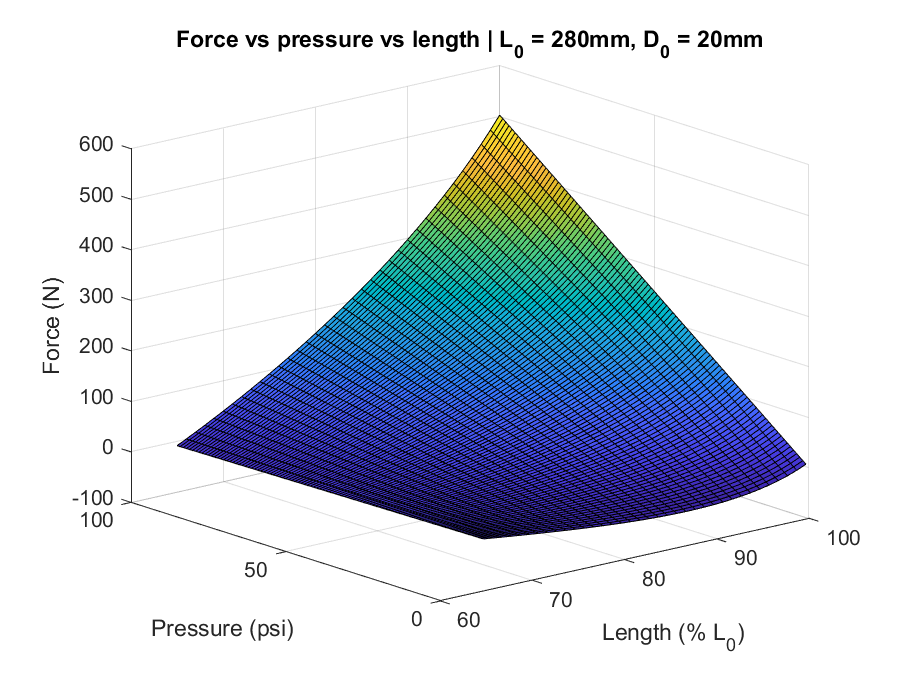
\includegraphics[scale=0.6]{staticmap.eps}
    \label{fig:staticmap}
\end{figure}

\subsubsection{Dynamic Modelling}
\label{sub:dynamic_modelling}
Pneumatic air muscles have their own dynamics, like hysteresis, some thermodynamic effects and can even be interpreted as a mass spring damper combination \cite{martens_boblan_2017}. Models dependent on the construction parameter and air pressure have been developed providing a tensile force formula of the contractor actuator and can be modified to describe the extension force. One model based on a combination of sigmoid functions representing the force output as a function of both the air pressure and initial length, is an estimation derived from three experimental results over varying lengths. This model assumes an average extension ratio of 50\%, the perfect cylindrical shape with zero wall thickness of the inner bladder, constant friction-less contact between the braid and inner tube, constant braid strand length and elasticity of the rubber tube. This model lacks an accurate description of the complex non-cylindrical shape at low pressures and the imperfect contact between the inner tube and braided sleeve \cite{al-ibadi_nefti-meziani_davis_2018}. \newline

Extending this the problem can be approached firstly as a mechanically derived nonlinear spring, the stiffness of which can be controller by the muscle pressure. This relationship can be depicted by a fifth order polynomial of two variables of 21 coefficients. The pneumatic part of the model is divided into two main components, the model of volume flow rate through the valves and a differential equation for the muscle pressure. The use of on/off style solenoid valves simplifies the flow rate to either a constant compressor pressure or atmospheric pressure, solely dependent on the muscle pressure. The second pneumatic component is the derivative time dependent equation derived from ideal gas laws. This research found that the hysteresis effects of the muscle actuator cause some steady state error due to simplified descriptions of the mechanical force components. Refinement of the model could decrease the errors to reduce the reliance on the robustness of the control technique \cite{hosovsky_2012}. Below is the equation found representing these forces (\ref{math:dynamicforce}), where m - moving mass (kg), y - muscle displacement (m), F\textsubscript{S}(k,P\textsubscript{m}) - nonlinear term representing a variable spring force (N), F\textsubscript{D}(\.{k},P\textsubscript{m}) - nonlinear term representing a variable damper force (N), F\textsubscript{E} - external force (N), k - muscle contraction (defined as k = k\textsubscript{0} + y/l\textsubscript{0} where k\textsubscript{0} is the initial contraction and l\textsubscript{0} is the initial muscle length (-) and P\textsubscript{m} - the absolute muscle pressure (Pa).

\begin{equation}
    \ddot{y} = \frac{1}{m}[F_E-F_S(k,P_m)-F_D(\dot{k},P_m)]
    \label{math:dynamicforce}
\end{equation}

\newpage
\section{System Implementation}
\label{sec:system_implementation}

% You finally get to write about what you have done! \newline
% Should use and build upon the background material in the previous chapter (or it shouldn't have been there in that chapter in the first place!). \newline
% Long and tedious proofs, detailed descriptions of circuits or software, and other necessary but unreadable bits, should go in one or more appendices at the end of the thesis. \newline

% Implementation Aspects of .....
% How did you undertake the theoretical analysis/simulation/construction/software development? \newline 
% What did you build? \newline
% What software did you write? \newline
\subsection{Platform Design}
\label{sub:platform_design}
The ultimate goal of this design, dubbed PNEUbot, will be to develop a humanoid robotic platform designed to replicate the motions of a human closer than the current electric servo driven humanoid robots. To achieve this goal an alternate actuator must be developed and a platform feasibility study performed to determine the viability of the actuator developed. Shown in figure \ref{fig:platform} this platform has been designed to mimic the range of joint movements capable by a human, this biologically inspired platform is formed around the skeleton dimensions of an adult human, implementing muscle groups to control the joints for each degree of freedom. Due to the reduced contraction of pneumatic muscles 25-30\% compared to the 50-70\% stroke of a human muscle, design constraints needed to be placed on some DoF for the range of motion available for that joint. Consequently, due to the force curve produced by pneumatic muscles, the force capable of being produced at the end of a muscle stroke is limited by it's physical parameters. \newline

The current world class strictly humanoid robotic platform was designed by a German team from the University of Bonn. This platform stands 135cm tall, weights 18kg and has 18 DoF: 5 per leg (parallel kinematics), 3 per arm and 2 in the neck \cite{ficht_farazi_brandenburger_rodriguez_pavlichenko_allgeuer_hosseini_behnke_2018}. These servos are capable of producing 12.9 N.m of stall torque with a maximum rpm of 37 at no load at a 12 bit resolution \cite{robotis}. For this project, this platform will be the benchmark for the use of pneumatic air muscles as an alternate actuator. \newline

\begin{figure}[hbt!]
    \centering
    \begin{subfigure}[t]{0.4 \textwidth}
        \centering
        \caption{Side Profile}
        \includegraphics[scale=0.2]{Leg_Render_Side_2.PNG}
        \label{fig:platform_side}
    \end{subfigure}
    \begin{subfigure}[t]{0.4 \textwidth}
        \centering
        \caption{Design Concept}
        \includegraphics[scale=0.2]{Leg_Render.PNG}
        \label{fig:platform_angle}
    \end{subfigure}
    \caption{PNEUbot Robotic Platform Concept Design}
\end{figure}

To achieve a lightweight skeleton the robot will be constructed from aluminium extrusion 'bones', 3D printed mounts and protective covers. Bearings will be inserted into the knee joint, with a spherical ball joint forming the ankle pivot. High tensile nylon line will act as tendons providing the transmission of the pneumatic muscle force to the actuated joint. \newline

The knee joint will consist of a pair of muscles acting as the flexion and extension muscles. These will be placed on the upper leg area of the robot producing approximately 120$^{\circ}$ of motion. To achieve the 2 DoF dorsiflexion/plantar flexion and everision/inversion of the ankle, a 2 pairs of coupled muscle actuators will be placed around the lower leg. These muscles will be coupled as opposed to decoupled to provide a parallel actuation force for the plantar flexion of the ankle joint. This should theoretically reduce the force required from each muscle and thus the size of the muscles contained in the lower leg. 

\subsection{Muscle Construction}
\label{sub:muscle_construction}
% \newline TODO - talk about muscle construction and materials chosen \newline
The pneumatic muscles are constructed from two major components, the inner bladder and the outer braided mesh. The inner bladder was chosen with an internal diameter of 6mm and wall thickness of 1.5mm, this is due to the availability and cost factors for initial testing and will likely be increased. The braided mesh of 20mm diameter was selected to be compatible with the bladder diameter as according to \cite{andrikopoulos_nikolakopoulos_2017}.

\subsection{Pneumatic Control}
\label{sub:pneumatic_control}

In order to control the flow of air into and out of the muscle bladder a 3 port 2 way pneumatic solenoid valve was used in conjunction with a non-return valve \cite{airsky_pneumatic}. These components were assembled as shown in figure \ref{fig:pneumatic_valve}, this arrangement allows each muscle to be in 1 of 2 states which some transitions states occurring.

\begin{figure}[hbt!]
    \centering
    \caption{Single Muscle Actuator Assembly}
    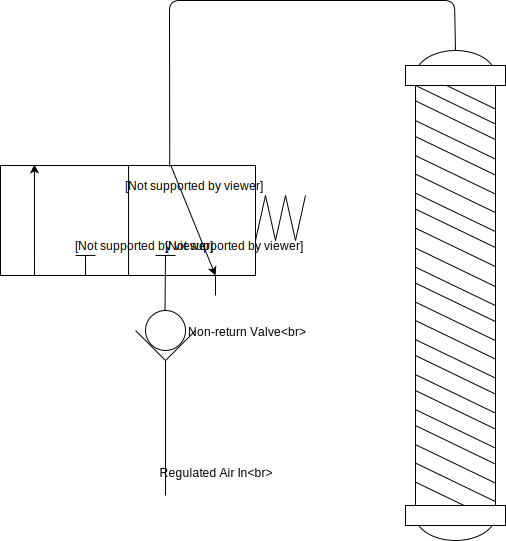
\includegraphics[scale=0.3]{Pneumatic_Design.png}
    \label{fig:pneumatic_valve}
\end{figure}

Consider one muscle under no load when its internal pressure is equal to the regulated system pressure, the muscle will be under full contraction. Releasing the air from the muscle will allow the muscle to extend back to its nominal length. Switching between the two valve states will allow the muscle to contract and release. Now consider the case where two muscles of equal parameters are appended end to end. Starting with both muscles at equilibrium pressure, regulated system pressure, the contraction percentage of both muscles will be equal. Switching the first muscle into the open position will allow the air to release from that muscle, this also allows the second muscle to contract filling with air. When the required position is reached the first muscle can be switched closed, causing the muscle to re-pressurise stopping the contraction of the second muscle. If the non-return valve was not installed, the system would be able to equalise the pressure between the two muscles when the force generated by each muscle was different due to the different contraction percentages. These states are similar to the SMC3 modes, however, the use of two valves per pair of muscles instead of four reduces the cost of the valves for the system. This also means that a SMC7 implementation is not possible, due to the limited number of states that the valve positions can form.

\subsection{Sensors}
\label{sub:sensors}
\newline TODO - section on sensors and sensor selection, pressure and linear pot
To measure the states of the system, pressure and linear position, a pressure sensor and linear potentiometer have been chosen. The pressure sensor is placed after the valve on the muscle side of the actuator. This pressure sensor \cite{} allows XXXXX bit resolution from XXX to XXX psi, and was attached to a custom pcb that provides a differential reading of the sensor to be fed into the micro controller. A rotary potentiometer or encoder could have been used for the axial position measurement and placed on the rotational axis of each joint, however, the design and construction for the 2 DoF ankle joint would be more complex. This then lends itself to the use of linear potentiometers attached to the end of each muscle, eliminating the need to a sensor attached directly to the rotational axis.

\subsection{Microcontroller}
\label{sub:microcontroller}
\newline TODO - talk about the NUCLEO mcu chosen for the number of ADC channels and speed \cite{stm32_nucleo_stm32f722ze}

\subsubsection{Electronics Shield}
\label{sub:shield}
\newline TODO - shield board designed to power the valves and perform the interface to the sensors

\subsubsection{Software}
\label{sub:software}
\newline TODO - talk about the software developed to perform the sensor readings and processing

\newpage
\section{Testing and Evaluation}
\label{sec:results}

% What it showed and/or failed to show. Did it work as expected? Why might it have gone
% wrong? 
\subsection{Static Map}
\label{sub:static_map}
TODO - What i did. Static map, compared to papers map/predicted. How this will be used later.
\subsection{Step Response}
\label{sub:step_response}
TODO - Step response, how this is bad over large changes, but alright over small ones

\newpage
\section{Conclusion}
\label{sec:conclusion}

\newline TODO - Conclusions summarises what you set out to do, how you did it, and how it worked or didn't work (and don't believe it has to work to make it a worthwhile project - you
have to work, the project doesn't!). Should be about two pages, and can be "cut and
pasted" from earlier chapters.


\newpage
\section{Further Work}
\label{sec:further}

% Extensions : Look at it this way - if you inherited this project from someone else,
% you'd like to be given some guidelines as to what to do and what not to do, from here
% on. What additions, modifications could/should be tried?
\newline TODO - Construction of the full platform prototype (leg)
\newline TODO - Implementing non linear control scheme

\newpage

\section{Appendix}
\label{sec:appendix}
\subsection{Appendix A}
\label{sub:staticforcederive}
Approximating the volume as a cylinder, the dependency of the diameter on the length can be approximated by using the Pythagoras theorem 
\begin{equation}
    D(L) = \frac{\sqrt{L_{Fiber}^2-L^2}}{n \pi}
\end{equation}
This then follows that equations \ref{math:diameterconst1} and \ref{math:diameterconst2} are only dependent on the initial conditions
\begin{equation}
    n = \frac{L_0tan(\Theta_0)}{\pi D_0}
    \label{math:diameterconst1}
\end{equation}
\begin{equation}
    L_{Fiber} = \frac{L_0}{cos(\Theta_0)}
    \label{math:diameterconst2}
\end{equation}
Inserting the functional dependency on the diameter into the equation of a cylinder results in a volume only dependent on the length and initial conditions
\begin{equation}
    V(L) = \frac{L L_{Fiber}^2}{4 \pi n^2}-\frac{L^3}{4 \pi n^2}
\end{equation}
The virtual work of the PMA can be split into two parts, the work done by the volume of air and the elasticity of the membrane 
\begin{equation}
    W_{PMA} = W_{VAE} + W_{Elast}
\end{equation}
\begin{equation}
    \sigma_{L} = E_{RU}(L) \frac{L-L_0}{L_0}
\end{equation}
\begin{equation}
    \sigma_{PE} = E_{RU}(L) \frac{D-D_0}{D_0}
\end{equation}
\begin{equation}
    W_{L} = -\sigma_{L} H_0 \pi D(L)
\end{equation}
\begin{equation}
    W_{Elast-PE} = -\sigma_{PE} H_0 L \pi
\end{equation}
Finally the following equation gives the positive pulling force exhorted by the muscle
\begin{equation}
    F_{PMA}(\rho, l) = -\rho \frac{dV}{dL}+F_{PE} \frac{dD}{dL}-F_L
    \label{math:staticforcederive}
\end{equation}

\newpage

%%% Display the bibliography.
\printbibliography
\end{document}